%This work is licensed under the Creative Commons License Attribution 4.0 International (CC-BY 4.0)
%https://creativecommons.org/licenses/by/4.0/legalcode
\documentclass[rgb]{standalone}
\usepackage{tkz-euclide}
\usepackage{amsmath}
\definecolor{myorange}{hsb}{0.0833, 1, 0.8}
\definecolor{mygreen}{hsb}{0.3333, 1, 0.8}
\definecolor{myblue}{hsb}{0.5833, 1, 0.8}
\definecolor{mymagenta}{hsb}{0.8333, 1, 0.8}
\begin{document}
	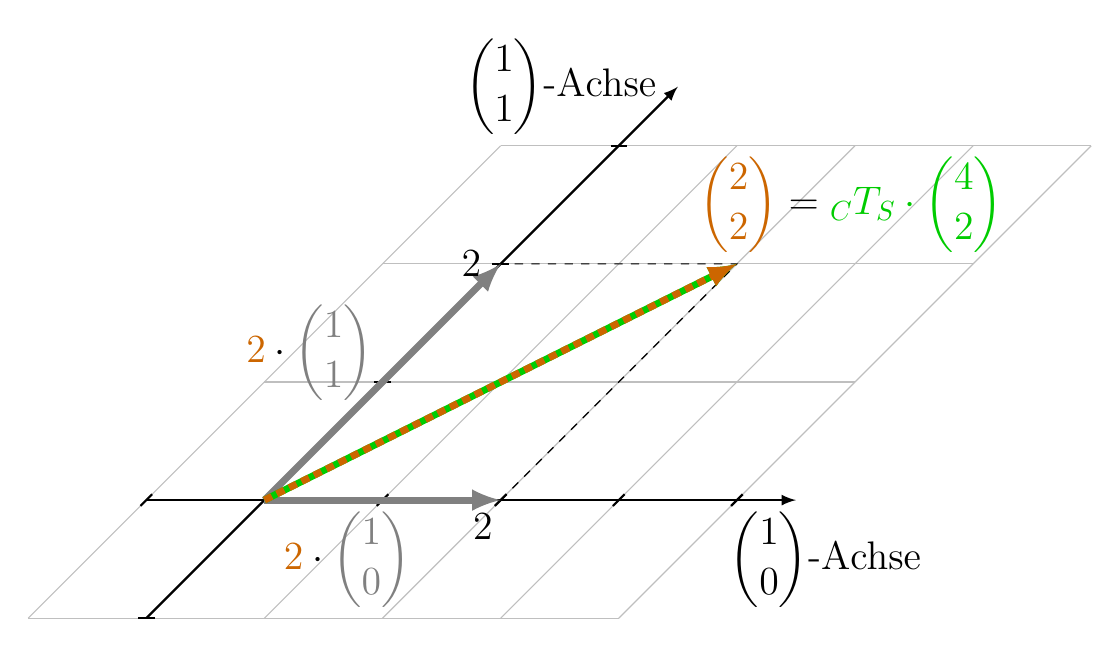
\begin{tikzpicture}[scale=1.5, font=\Large]
		\foreach \i in {-1,1,2,3}
		{			
			\draw[lightgray] (-1+\i,\i) -- (4+\i,\i);
			\draw[thick] (-0.07+\i,\i) -- (0.07+\i,\i);
		}
		\foreach \i in {-1,1,2,3,4}
		{
			\draw[lightgray, rotate=-45] ({\i*0.5*sqrt(2)},{-sqrt(2)+\i*0.5*sqrt(2)}) -- ({\i*0.5*sqrt(2)},{3*sqrt(2)+\i*0.5*sqrt(2)});
			\draw[thick, rotate=-45] ({\i*0.5*sqrt(2)},{-0.07+\i*0.5*sqrt(2)}) -- ({\i*0.5*sqrt(2)},{0.07+\i*0.5*sqrt(2)});
		}
		\draw[thick, -latex] (-1,0) -- (4.5,0);
		\draw[thick, -latex, rotate=-45] (0,{-sqrt(2)}) -- (0,{3.5*sqrt(2)});
		\draw[dashed] (2,0) -- (4,2) -- (2,2);
		\draw[line width=2.5pt, gray, -latex] (0,0) -- (2,0);
		\draw[line width=2.5pt, gray, -latex] (0,0) -- (2,2);
		\draw[line width=2.5pt, mygreen, -latex] (0,0) -- (4,2);
		\draw[line width=2.5pt, myorange, densely dashed, -latex] (0,0) -- (4,2);
		\node[below] at (4.75,0){$\begin{pmatrix} 1 \\ 0 \end{pmatrix}$-Achse};
		\node[left] at (3.4,3.5){$\begin{pmatrix} 1 \\ 1 \end{pmatrix}$-Achse};
		\node[below=0.5mm] at (1.85,0) {$2$};
		\node[left=0.5mm] at (1.95,2) {$2$};
		\node[above right] at (3.6,2){${\color{myorange}{\begin{pmatrix} 2 \\ 2 \end{pmatrix}}}=\color{mygreen}{{}_{C}T_{S}\cdot\begin{pmatrix} 4 \\ 2 \end{pmatrix}}$};
		\node[below] at (0.7,0){${\color{myorange}{2}}\cdot\color{gray}{\begin{pmatrix} 1 \\ 0 \end{pmatrix}}$};
		\node[left] at (1,1.25){${\color{myorange}{2}}\cdot\color{gray}{\begin{pmatrix} 1 \\ 1 \end{pmatrix}}$};
	\end{tikzpicture}	
\end{document}